\section{Implementation}
\label{sec:implementation}
\subsection{Overview}
The implementation of our experiment contains three components. First, the implementation of the gossip-based aggregation is clarified. Next, the network emulation context is presented. Finally it is shown under which conditions the experiment was run.

\subsection{Implementation of gossip-based aggregation daemon}
As the gossip agent in our emulated network we developed a daemon based on the pseudo code of the gossip-based aggregation algorithm (see section \ref{sec:theory}). The programming language Python \cite{python} was chosen for this task as its simplicity and clarity enable a rapid development. Packets between nodes were exchanged in short lived TCP connections. The daemons on the individual nodes are started from outside the emulation system and write a log and results to the host system. After a number of epochs (successive fixed intervals) the daemons exit.

Two threads are coexisting (see figure \ref{fig:flow_diag}). The active thread connects to randomly chosen neighbors at a epoch duration. The passive thread accepts connection all the time. Each thread update the state of the node after a successful connection. To make the state develop linearly both threads have to compete for a lock before establishing a connection. \footnote{Combining multithreading with networking led to some problems, especially when two nodes chose to actively create a connection with each other at the same time.}
\begin{figure}[h!]
    \begin{center}
        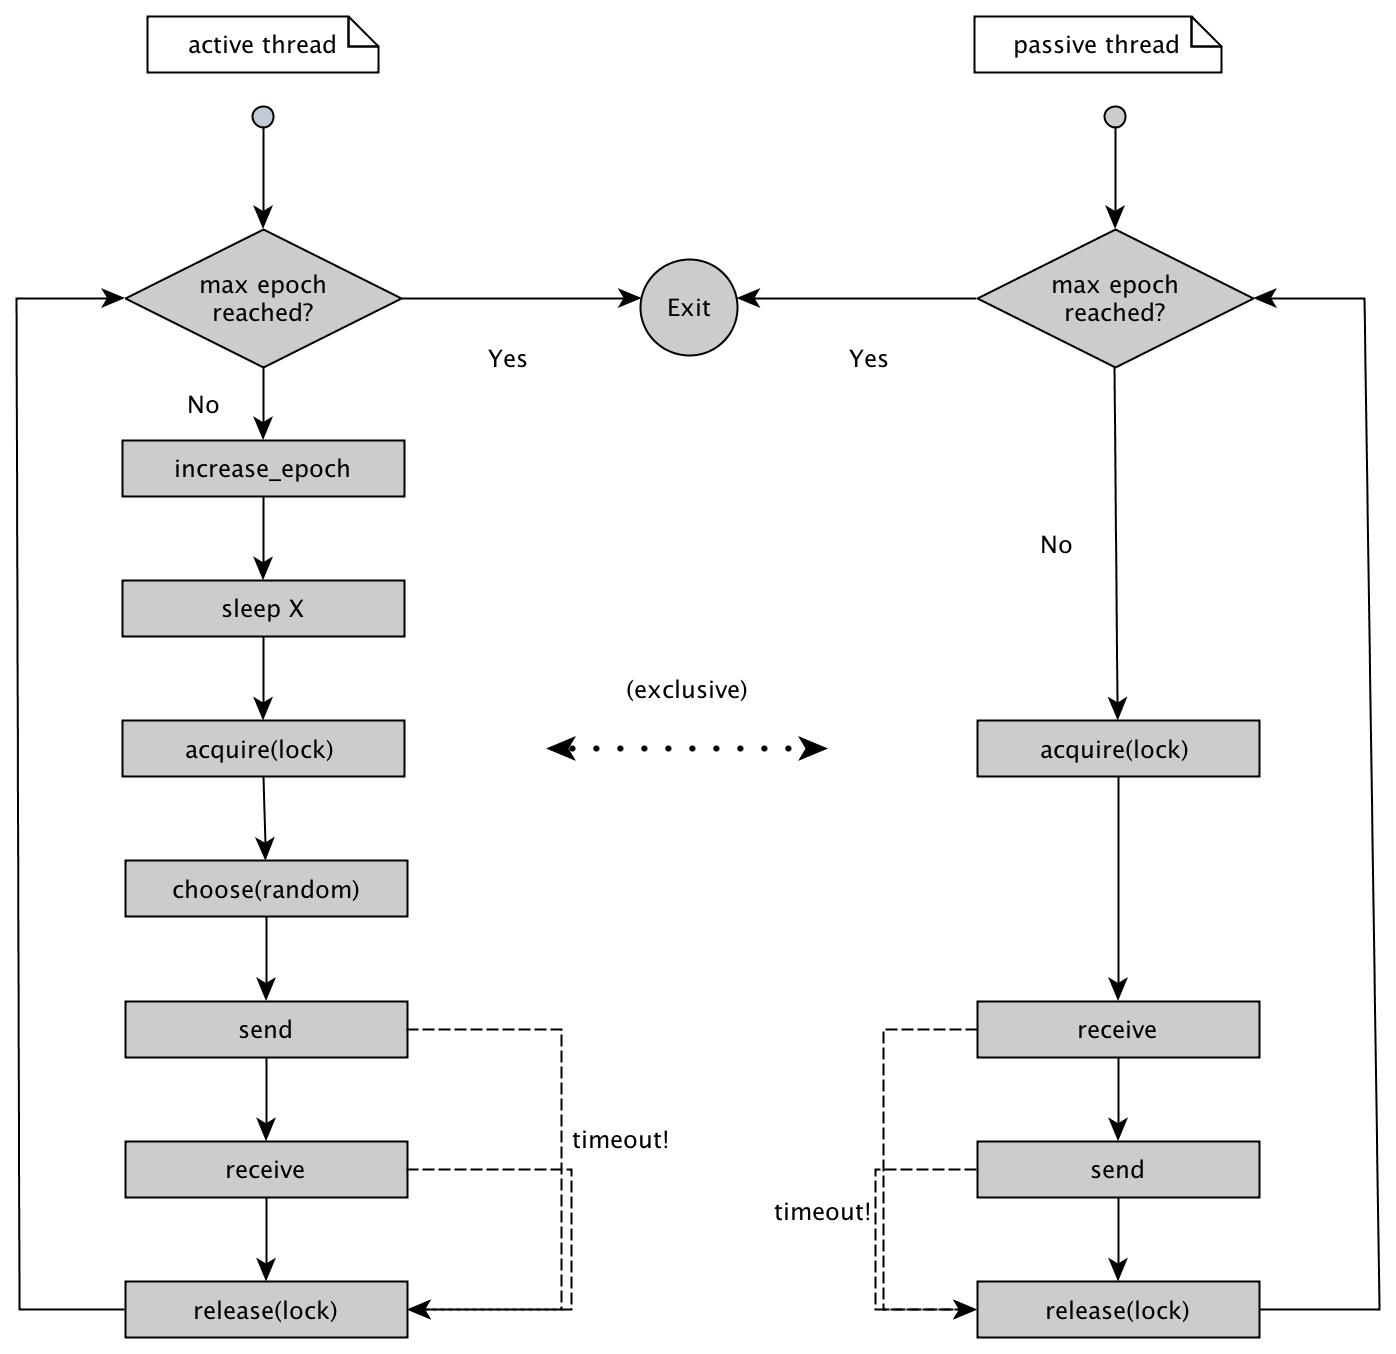
\includegraphics[scale=0.25]{flow_diag.jpg}
    \end{center}
    \caption{Flow diagram of the threads}
    \label{fig:flow_diag}
\end{figure}

Data created this way over one graph is analyzed in R. We compare our four different topologies (mentioned above) and visualize the results as charts. The code of our program as well as the results below are available at github: \url{https://github.com/metaswirl/py_gossip}

\subsection{Simulation of gossip-based aggregation}
In a network simulation the network is simplified so as to illuminate a certain set of behaviors (e.g. Network Simulator \cite{ns}). For the purpose of simulation, gossip-based aggregation in one epoch is abstracted as a pair choosing process: in every epoch, every node is iterated exact once and one of its neighbor is randomly chosen to form a state exchange pair, and then aggregation operation, in this case add and divide by two, is applied. In this manner, convergence and different behaviors of four topologies can be predicted without running the actual emulation.
\subsection{Emulation of gossip-based aggregation}
The aim of our experiment is to evaluate gossip based aggregation for real world computer networks. To this end the gossip-based aggregation has to be implemented over a computer network. Unfortunately the setup of a real network is too time and cost intensive. Hence the next best thing was chosen: A network emulation. 
An emulation consists of all the elements of the real network only that the resources are not "real" but "virtual". While for example an emulated switch may process network traffic in the very same way as a switch in your office, it could be implemented as a linux process.

\begin{figure}[h!]
    \begin{center}
        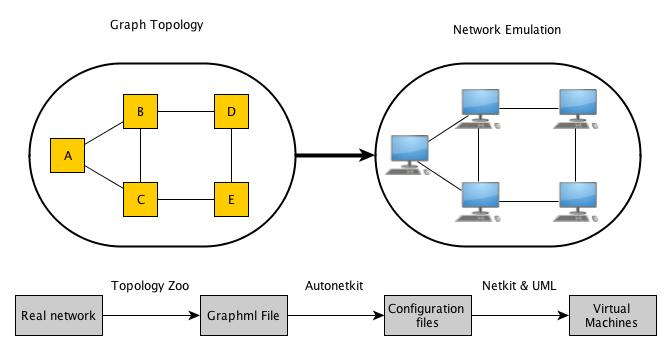
\includegraphics[scale=0.6]{graph_to_emulation}
    \end{center}
    \caption{From a graph to an emulated network}
    \label{fig:graph_to_emulation}
\end{figure}

In this research the Netkit emulation framework (itself a wrapper to user mode linux \cite{uml}) was chosen. Netkit \cite{netkit} creates virtual linux machines from a set of configuration files. These virtual machines are automatically connected through usermode processes called "uml\_switch". It is possible to log on to the machines via ssh and configure them just like any other linux machines. This allows great freedom to try and test software which otherwise would be hard to implement.

The initial set of configuration files were created with the tool Autonetkit \cite{autonetkit} using network graphs from the "Topology Zoo" \cite{knight_internet_2011}. The "Topology Zoo" is a collection of around two hundred fifty graphs of telecommunication networks. The graphs are open for use and give a good idea on the reality of communication networks. Simon Knight, one of the founders of the topology zoo has developed the tool Autonetkit. It takes a graph xml file (graphml) and constructs over a series of abstractions configuration files (from OSPF to DNS). For the purpose of this experiment Autonetkit was augmented so as to create for our gossip agent a file containing all neighbors of the individual nodes.

\subsection{Running the experiment}
The experiment was run on a host with 64 cores, each with 2299 MHz and 126GB of memory. Each virtual machine required 32Mbs of memory. The operating system was Ubuntu 11.10.
